\subsection{Word segmentation}
\label{sec:segmentation}


Does the model develop an implicit notion of word?

English/German/Italian

How validation partition was used

Use only one of the low-parameter-count methods, compare to Bayes
although it's not entirely fair (clarify that). (report in text or
footnote that, when training on the hidden state, we get super-high
accuracy, indicating that the information is there).

LSTM vs RNN vs Bayes vs n-gram baseline (collect transition
probabilities across fixed n-gram windows, optimize threshold on
validation data).

Results could be summarized as in Table \ref{tab:segmentation-results}.


\begin{table}[t]
  \begin{center}
    \begin{tabular}{l|l|l|l|l}
      \multicolumn{1}{c}{}&\emph{LSTM}&\emph{RNN}&\emph{Bayes}&\emph{ngrams}\\
      \hline
      English &\ldots{}/\ldots{}/\ldots & \ldots{}/\ldots{}/\ldots & \ldots{}/\ldots{}/\ldots &\ldots{}/\ldots{}/\ldots\\
      German &\ldots{}/\ldots{}/\ldots & \ldots{}/\ldots{}/\ldots & \ldots{}/\ldots{}/\ldots &\ldots{}/\ldots{}/\ldots\\
      Italian &\ldots{}/\ldots{}/\ldots & \ldots{}/\ldots{}/\ldots & \ldots{}/\ldots{}/\ldots &\ldots{}/\ldots{}/\ldots\\
    \end{tabular}
  \end{center}
  \caption{\label{tab:segmentation-results} Scores are P/R/F\ldots too packed?}
\end{table}



\begin{figure}
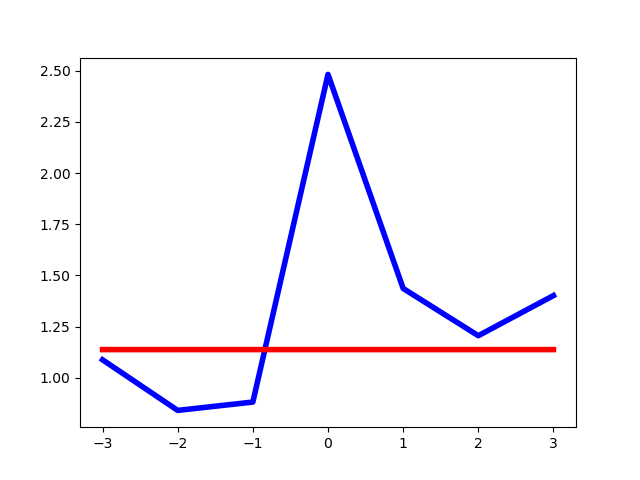
\includegraphics[width=0.22\textwidth]{figures/segmentation-profile-flattened-entropies-german.png}
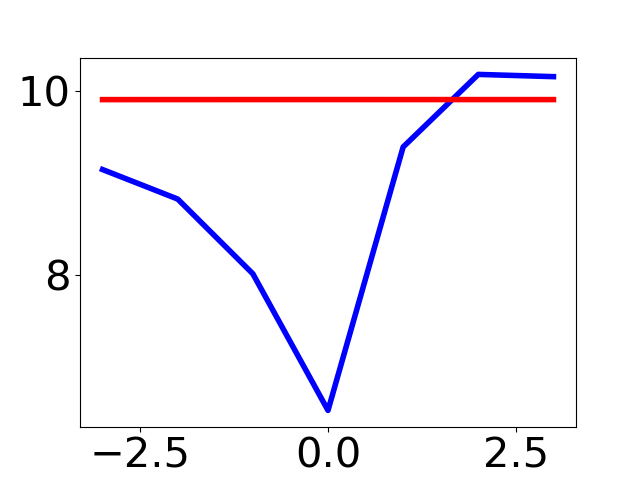
\includegraphics[width=0.22\textwidth]{figures/segmentation-profile-flattened-pmis-german.png}
	\caption{Entropy and PMI at word boundaries (blue), compared to all positions (red). }\label{fig:syntax-depth}
\end{figure}





We hypothesized that the same might be true for hierarchical syntactic structure.
We created constituency trees for the German validation set using the Berkeley Parser~\ref{petrov2007improved}.
For each character in the data, we counted its hierarchical distance from the preceding character, operationalized as the number of intervening closing and opening brackets.
This number is zero if both characters belong to the same word.

Figure~\ref{fig:syntax-depth} plots MI by height.
The plot shows that longer hierarchical distance between neighboring characters corresponds to lower average MI.
This illustrates how it is useful for
segmentation knowledge to be implicit, as the model ``knows'' about
different kinds of boundaries in a continuous manner.



\begin{figure}
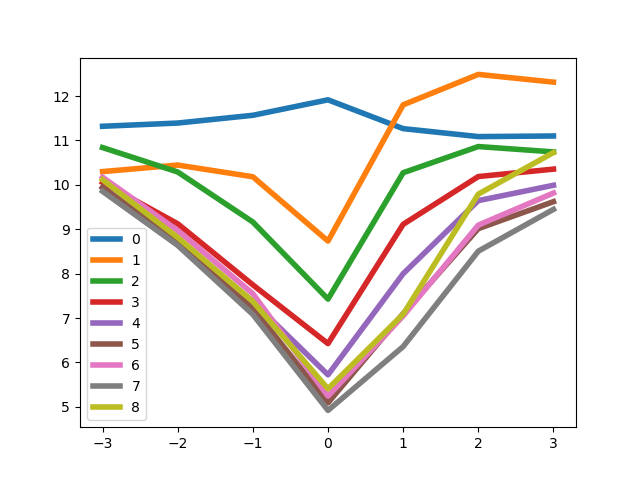
\includegraphics[width=0.48\textwidth]{figures/segmentation-profile-pmis-german-all-heights.png}
\caption{PMIs by syntactic depth.}\label{fig:syntax-depth}
\end{figure}




Qualitative analysis: report proportions of over- and
under-segmentation for our best CNLM, look at common over- and
under-segmentation errors in English (Marco will go manually
through the top 30 most common errors of both types).
